\section{Classification of Bd and Bs mesons}

The distinction of $B_d$ and $B_s$ mesons based on the associated event is a non-trivial problem.
Since both mesons have different masses, it is expected that there is some difference in the kinematics of the associated event.
Therefore, it is tested if a multivariate machine learning algorithm can spot these differences.
The algorithm of choice for this thesis is a DeepSet that is trained on simulated LHCb data.

The procedure of selecting important features is similar to the procedure described in \autoref{sec:SS_classifier}.
However, the feature importances used here are the permutation importance of the ROC AUC and the permutation importance of the accuracy.
Again, features with the lowest feature importance scores are discarded until a reasonable amount of features is achieved.
The remaining 23 features are listed in \autoref{tab:B_features} and the corresponding feature importances are shown in \autoref{fig:B_importances}.

\begin{figure}
    \centering
    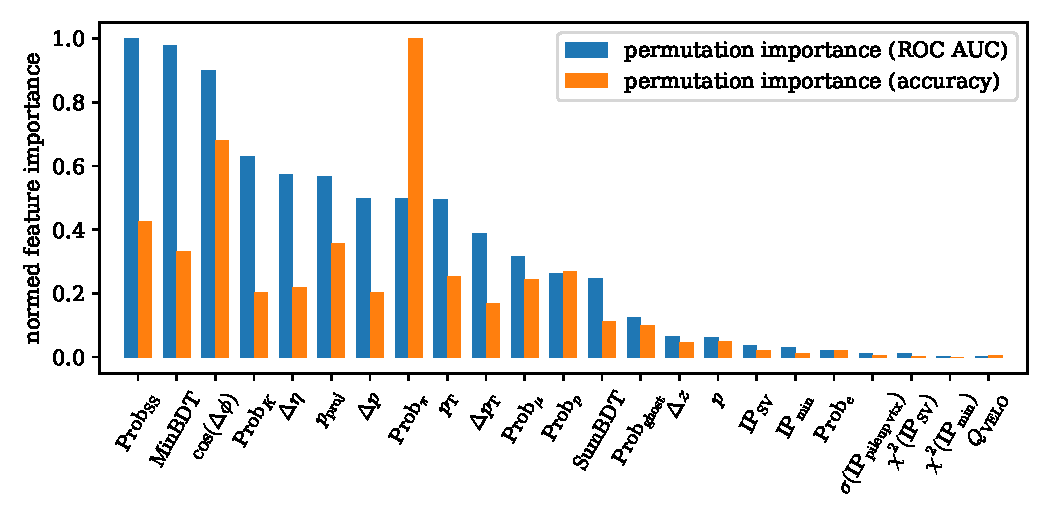
\includegraphics[width=\textwidth]{images/B_feature_importances.pdf}
    \caption{Calculated feature importances on the trained DeepSet. Shown are the permutation importances of the ROC AUC and the accuracy.}
    \label{fig:B_importances}
\end{figure}

\begin{table}
    \centering
    \caption{List of all features used to train the DeepSet for B meson classification.}
    \label{tab:B_features}
    \begin{tabular}{c c}
        \toprule
        feature & feature \\
        \midrule
        $p$                 & $\text{Prob}_\text{SS}$ \\ %"Tr_T_P","Tr_ProbSS"
        $p_\text{T}$        & $\text{PROBNN}_e$ \\ %"Tr_T_PT", "Tr_T_PROBNNe"
        $p_\text{proj}$     & $\text{PROBNN}_\text{ghost}$ \\ %"Tr_p_proj","Tr_T_PROBNNghost"
        $\Delta p_\text{T}$ & $\text{PROBNN}_k$ \\ %"Tr_diff_pt", "Tr_T_PROBNNk"
        $\Delta p$          & $\text{PROBNN}_\mu$ \\ %"Tr_diff_p","Tr_T_PROBNNmu"
        $\Delta z$          & $\text{PROBNN}_p$ \\ %"Tr_diff_z", "Tr_T_PROBNNp"
        $\cos(\Delta \phi)$ & $\text{PROBNN}_\pi$ \\ %"Tr_cos_diff_phi", "Tr_T_PROBNNpi"
        $\Delta \eta$       & IP\_trPUS \\ %"Tr_diff_eta", "Tr_T_IP_trPUS"
        IP\_trMother        & VeloCharge \\ %"Tr_T_IP_trMother",  "Tr_T_VeloCharge"
        IPCHI2\_trMother    & SumBDT\_ult" \\ %"Tr_T_IPCHI2_trMother", "Tr_T_SumBDT_ult"
        MinIP               & MinBDT\_ult \\ %"Tr_T_MinIP", "Tr_T_MinBDT_ult"
        MinIPChi2           & \\ %"Tr_T_MinIPChi2"
        \bottomrule
    \end{tabular}
\end{table}

(Explain all features)....
